%%
%% Author: Dario Chinelli
%% begin 2019-12-04
%% last mod 2022-02-02
%%

% Preamble
\documentclass[class=article, crop=false]{standalone}

% Packages
\usepackage{tikz}
\usetikzlibrary{positioning}

% Document
\begin{document}

\begin{figure}[h]
\centering
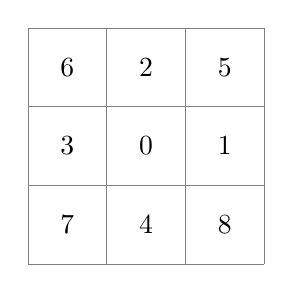
\begin{tikzpicture}
% Lines
\draw[step=1cm, gray, very thin] (0,0) grid (3,3);
% Nodes
\draw (1.5,1.5) node[black] {0};
\draw (2.5,1.5) node[black] {1};
\draw (1.5,2.5) node[black] {2};
\draw (0.5,1.5) node[black] {3};
\draw (1.5,0.5) node[black] {4};
\draw (2.5,2.5) node[black] {5};
\draw (0.5,2.5) node[black] {6};
\draw (0.5,0.5) node[black] {7};
\draw (2.5,0.5) node[black] {8};
\end{tikzpicture}
\captionsetup{width=.5\linewidth}
\caption{Transitions associated to possible movements from the center cell. The figure identify the $k$ nine values for each cell.}
\label{fig:D2Q9_k}
\end{figure}


\end{document}
